% !TEX program = xelatex
\documentclass[aspectratio=169,11pt]{beamer}
\usepackage[T1]{fontenc}
\usepackage{newtxtext,newtxmath,booktabs,graphicx}
\definecolor{Ink}{HTML}{101C34}
\definecolor{Cobalt}{HTML}{315DF6}
\definecolor{Copper}{HTML}{BE7132}
\definecolor{Muted}{HTML}{536174}
\setbeamercolor{normal text}{fg=Ink,bg=white}
\setbeamercolor{frametitle}{fg=Ink}
\setbeamercolor{structure}{fg=Cobalt}
\setbeamercolor{itemize item}{fg=Cobalt}
\setbeamerfont{frametitle}{family=\rmfamily,size=\LARGE,series=\bfseries}
\setbeamertemplate{navigation symbols}{}
\setbeamertemplate{footline}{\hfill\color{Muted}\scriptsize\insertframenumber\hspace{5mm}\vspace{3mm}}
\setbeamersize{text margin left=8mm,text margin right=8mm}
\setbeamertemplate{frametitle}{\vspace{5mm}\insertframetitle\par\vspace{4mm}}
\newcommand{\source}[1]{\vfill{\tiny\color{Muted}#1}}
\title{TrustVerify}
\author{BAHODIR KODIRJON UGLI NAZAROV}
\date{November 2026}
\begin{document}
{\setbeamercolor{background canvas}{bg=Ink}\setbeamercolor{normal text}{fg=white}
\begin{frame}[plain]
\color{white}\vspace{6mm}{\Huge\bfseries TrustVerify}\par\vspace{8mm}
{\LARGE Executable Verification of\\AI-Generated Data Analysis}\par\vspace{14mm}
{\normalsize BAHODIR KODIRJON UGLI NAZAROV}\par\vspace{4mm}
{\small Sichuan University\\New Software Technology, November 2026}
\end{frame}}
\begin{frame}{A plausible report can contain a wrong result}
\begin{columns}[T]\begin{column}{.48\textwidth}{\Huge\color{Copper}266.71\%}\par\vspace{4mm}Reported percentage\end{column}
\begin{column}{.48\textwidth}{\Huge\color{Cobalt}263.46\%}\par\vspace{4mm}Independent recomputation\end{column}\end{columns}
\vspace{12mm}Same dataset and approved contract. The discrepancy is 3.25 percentage points.
\source{Controlled example: ratio-02, complete-case ratio of sums.}
\end{frame}
\begin{frame}{Verification follows an explicit contract}
\begin{enumerate}
\item Approve the operation, columns, unit and missing-value rule.
\item Independently recompute the expected result from the original CSV.
\item Compare the candidate's numbers, units, row count and chart data.
\item Return a pass, failure findings or an abstention.
\end{enumerate}
\vspace{5mm}The production checker uses Decimal. The independent evaluation oracle uses SQLite.
\source{Implementation: trustverify/core.py and trustverify/benchmark.py.}
\end{frame}
\begin{frame}{Sixty datasets across six analytical operations}
\begin{tabular}{lrr}\toprule Operation & Development & Test\\\midrule
Sum & 2 & 8\\Mean & 2 & 8\\Weighted mean & 2 & 8\\Ratio of sums & 2 & 8\\Grouped sum & 2 & 8\\Percentage change & 2 & 8\\\bottomrule\end{tabular}
\hfill\begin{minipage}{.42\textwidth}{\Huge\color{Cobalt}60}\par datasets\vspace{7mm}\par{\Huge 24}\par pilot tasks per model\end{minipage}
\source{Fixed seeds. Dataset-level split. Pilot uses four held-out tasks per operation.}
\end{frame}
\begin{frame}{Both repair branches receive one additional call}
\begin{tabular}{lp{.64\textwidth}}\toprule Condition & Available evidence\\\midrule
Initial answer & Task, source data and approved contract\\[3mm]
Self-review & Same inputs and the initial response\\[3mm]
Executable feedback & Same inputs and computed discrepancies\\\bottomrule\end{tabular}
\par\vspace{8mm}Two models $\times$ 24 tasks $\times$ three calls = \textbf{144 recorded calls}.
\source{Temperature 0, seed 31415, 4096 context tokens and 384 output tokens per call.}
\end{frame}
\begin{frame}{Full checking detects 85.7\% of controlled faults}
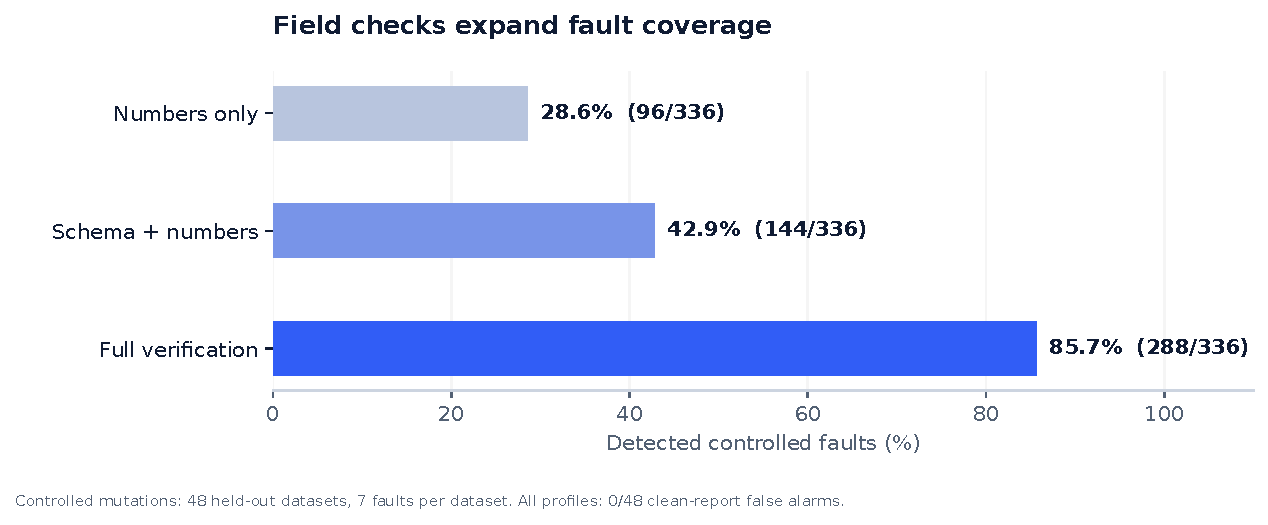
\includegraphics[width=.94\textwidth,height=.65\textheight,keepaspectratio]{../paper/figures/fault_coverage.pdf}
\source{288/288 supported structured faults detected. All 48 causal-prose faults remain outside scope.}
\end{frame}
\begin{frame}{Coverage depends on the field being checked}
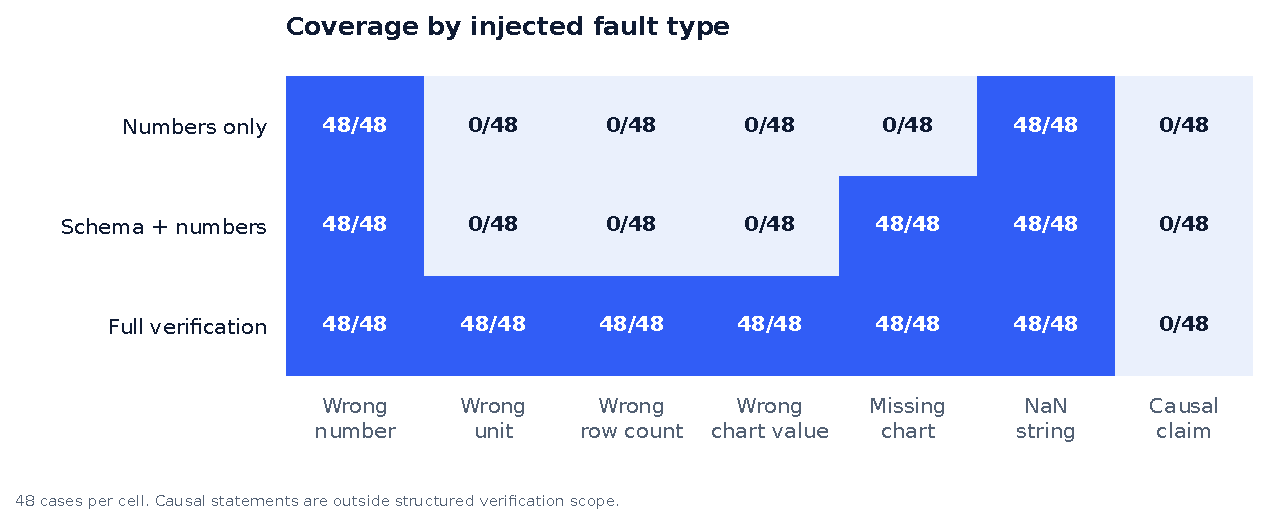
\includegraphics[width=\textwidth,height=.68\textheight,keepaspectratio]{../paper/figures/fault_matrix.pdf}
\end{frame}
\begin{frame}{Feedback repairs 19 of 24 numeric mappings}
\begin{columns}[T]\begin{column}{.47\textwidth}{\Huge\color{Cobalt}19/24}\par\vspace{5mm}Correct numeric mappings after executable feedback\end{column}
\begin{column}{.47\textwidth}{\Huge\color{Copper}0/24}\par\vspace{5mm}Fully correct reports after the same feedback\end{column}\end{columns}
\vspace{10mm}Numerical correctness is an exploratory endpoint. The primary endpoint requires every structured field to be correct.
\source{Qwen2.5 1.5B. Self-review produces 0/24 correct numeric mappings.}
\end{frame}
\begin{frame}{Grouped sums remain difficult after feedback}
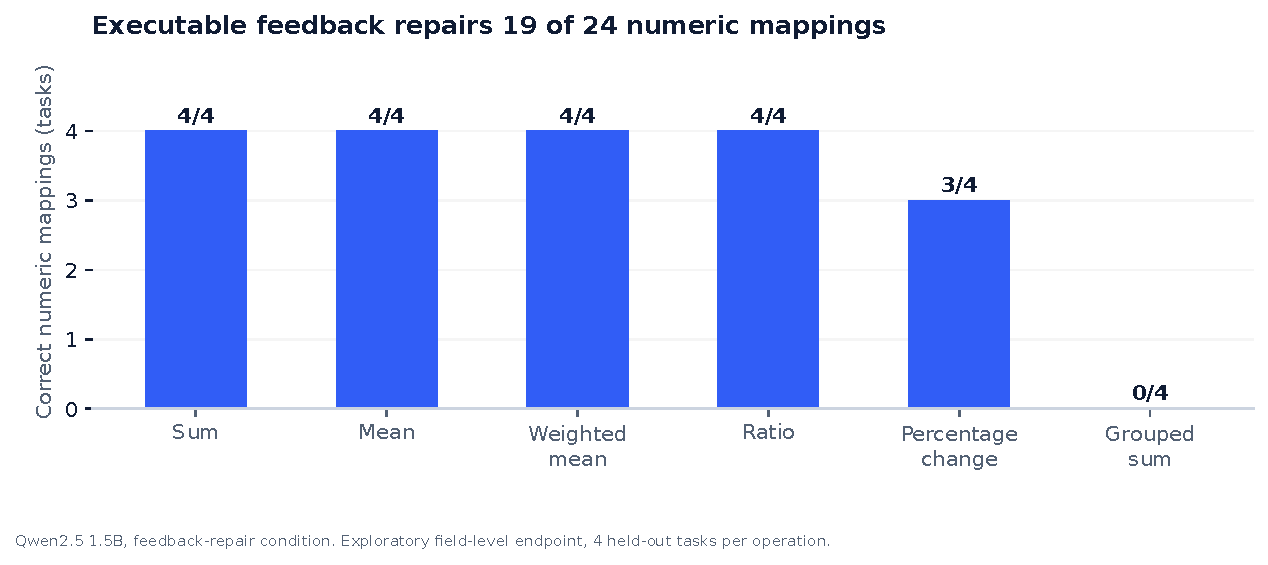
\includegraphics[width=\textwidth,height=.7\textheight,keepaspectratio]{../paper/figures/numeric_by_family.pdf}
\end{frame}
\begin{frame}{Chart consistency is the main output bottleneck}
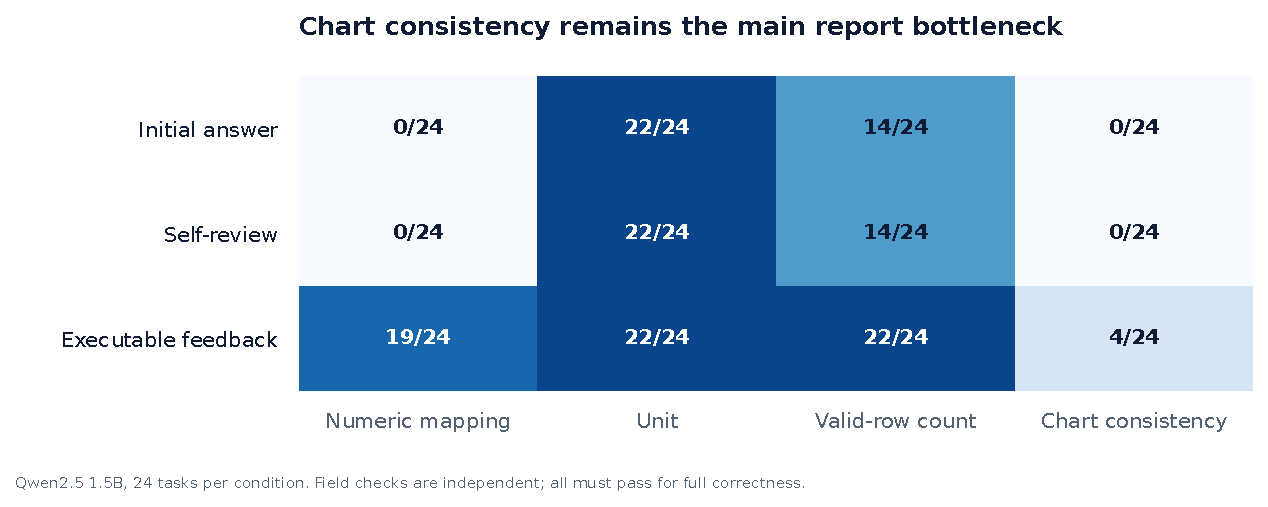
\includegraphics[width=\textwidth,height=.7\textheight,keepaspectratio]{../paper/figures/field_compliance.pdf}
\end{frame}
\begin{frame}{No generated report satisfies every field}
\begin{tabular}{lrrr}\toprule Model & Initial & Self-review & Feedback\\\midrule
Qwen2.5 0.5B & 0/24 & 0/24 & 0/24\\[4mm]
Qwen2.5 1.5B & 0/24 & 0/24 & 0/24\\\bottomrule\end{tabular}
\par\vspace{10mm}Each primary estimate has a descriptive 95\% Wilson interval of 0.0--13.8\%.
\source{Actual recorded model outputs. Deterministic recomputation is reported separately.}
\end{frame}
\begin{frame}{The local demo makes discrepancies inspectable}
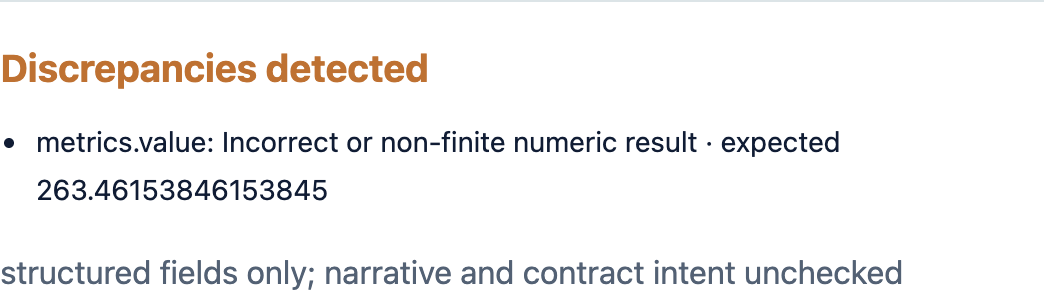
\includegraphics[width=.88\textwidth,height=.52\textheight,keepaspectratio]{../demo/checker-detail.png}
\vspace{4mm}\par\texttt{python3 -m trustverify.server}\\\texttt{http://127.0.0.1:8765}
\source{Actual interface capture. This example contains a controlled numeric mutation.}
\end{frame}
\begin{frame}{The verification boundary is explicit}
\begin{tabular}{lp{.62\textwidth}}\toprule Boundary & Remaining risk\\\midrule
Approved intent & Correct execution of the wrong operation\\[3mm]
Narrative meaning & Unsupported causal or contextual claims\\[3mm]
Data quality & Incorrect or unrepresentative source observations\\[3mm]
Chart appearance & Misleading axes despite consistent data values\\\bottomrule\end{tabular}
\source{Scope challenges are included in the controlled cases and test suite.}
\end{frame}
\begin{frame}{Independent execution repairs selected claims}
\noindent{\LARGE\color{Cobalt}288/336 controlled faults detected}\par\vspace{8mm}
{\LARGE\color{Cobalt}19/24 numeric mappings repaired}\par\vspace{10mm}
Reliable reporting requires independent computation and complete output validation.
\source{The findings apply to the documented operations, synthetic tasks and tested local models.}
\end{frame}
\begin{frame}{Research foundations and reproducibility}
\small
Jing et al. (2025). \textit{DSBench}. arXiv:2409.07703.\par\vspace{3mm}
Madaan et al. (2023). \textit{Self-Refine}. arXiv:2303.17651.\par\vspace{3mm}
Huang et al. (2024). \textit{Large Language Models Cannot Self-Correct Reasoning Yet}. arXiv:2310.01798.\par\vspace{9mm}
\normalsize\color{Cobalt}Source, datasets, raw responses and experiment evidence\par\vspace{3mm}
\small\url{https://github.com/naazzarov/trustverify-ai-analysis}
\end{frame}
\end{document}
